%Solucion del ejercicio por medio de la metodologia de las 6D

\subsection{Descripci\'{o}n del problema}
Dada una tabla de verdad de \textit{n} bits generar la expresión booleana que genere de manera fidedigna las salidas de esta tabla.

\subsection{Definici\'{o}n de la soluci\'{o}n}
Para llevar a cabo los teoremas booleanos, es necesario contar con datos específicos previamente obtenidos. Estos datos se obtienen a partir de una tabla de verdad que ha sido previamente creada y resuelta. Una vez que se disponen de los datos, es posible utilizar los teoremas booleanos con el fin de simplificar la expresión obtenida de la tabla de verdad, sin que esto afecte el resultado.

\subsection{Diseño de la soluci\'{o}n}

\begin {figure}[H]
\centerline{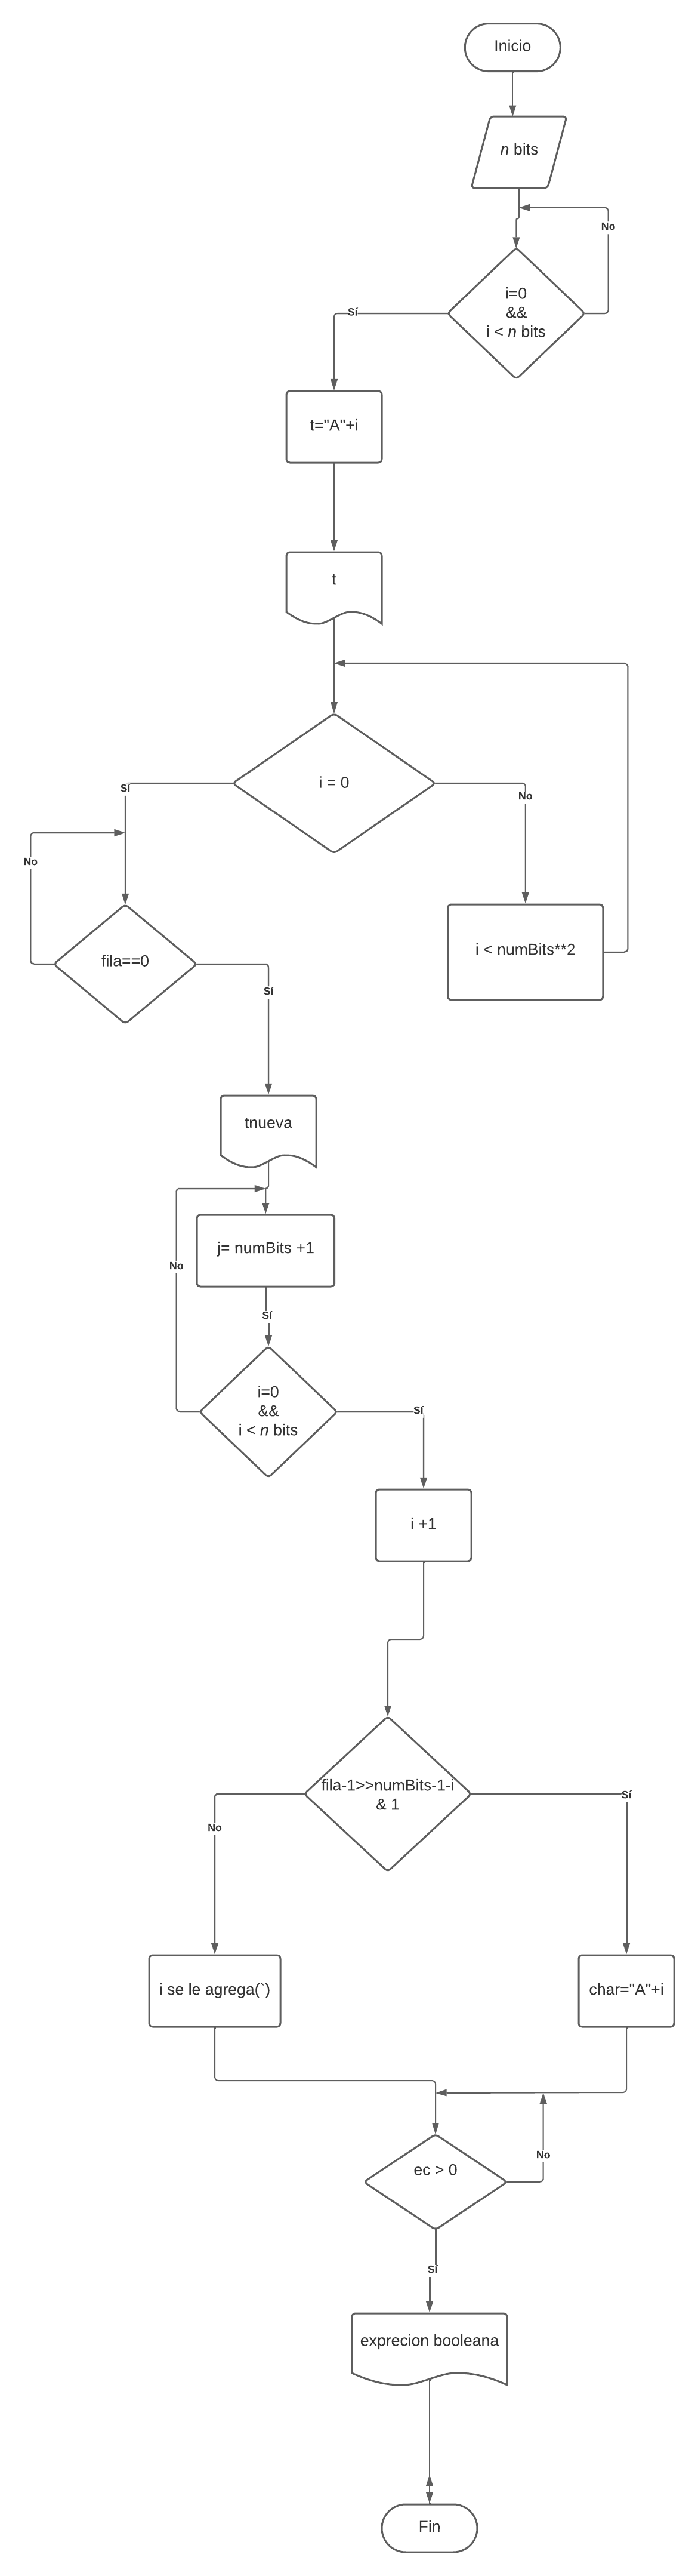
\includegraphics[width = 6cm]{Latex-imágenes/Diagrama de Tabla de Verdad (1).png}}
\caption{Diagrama de Tabla de Verdad del problema 6}
\label{fig}
\end {figure}

\subsection{Desarrollo de la soluci\'{o}n}
En el siguiente bloque de cod\'{i}go, se muestra una ventana donde pide al usuario que inserte el numero de bits.
\begin{javaCode}
     public static void main(String[] args) {
         Set<Integer> filasCambiar = new HashSet<>();
 
        String numBitsStr = JOptionPane.showInputDialog("Ingrese el Número de Bits que deberá ser la Tabla de Verdad:");
        int numBits = Integer.parseInt(numBitsStr);
\end{javaCode}

\subsection{Depuraci\'{o}n de las pruebas}

Ingrese el número de la fila que desea cambiar el resultado a 1 (1-8) o ingrese 0 para finalizar: 0
Expresiones booleanas al finalizar:
A' + B' + C'
A' + B' + C
A' + B + C
A + B' + C
A + B + C'
A + B + C.

Expresión booleana final: (A' + B' + C') + (A' + B' + C) + (A' + B + C) + (A + B' + C) + (A + B + C') + (A + B + C)


En la siguiente tabla se muestra lo antes explicado:

\begin{table}[h!]
  \centering
  \caption{Tabla de corridas para el Ejercicio 6.}
  \label{tab:tabla_ejemplo}
  \begin{tabular}{|l|c|r|c|}
    \hline
    \textbf{$A$} & \textbf{$B$} & \textbf{$C$} & \textbf{RESULTADO} \\
    \hline
    0 & 0 & 0 & 1\\
    0 & 0 & 1 & 1\\
    0 & 1 & 0 & 0\\
    0 & 1 & 1 & 1\\
    1 & 0 & 0 & 0\\
    1 & 0 & 1 & 1\\
    1 & 1 & 0 & 1\\
    1 & 1 & 1 & 1\\
    
    \hline
  \end{tabular}
\end{table}